\documentclass[10pt,a4paper]{article}
\usepackage[utf8]{inputenc}
\usepackage[russian]{babel}
\usepackage[OT1]{fontenc}
\usepackage{amsmath}
\usepackage{amsfonts}
\usepackage{amssymb}
\usepackage{graphicx}
\graphicspath{{lab5/}}

\author{Климов С.А., Назарова К.Е.}
\title{Отчет по лабораторным работам по дисциплине ТСС}
\date{2014}
\begin{document}
\maketitle
\pagebreak
\tableofcontents
\pagebreak
\section{Система верстки \TeX и расширения \LaTeX}
\subsection{Цель работы}
Изучение принципов верстки ТеХ, создание первого отчета
\subsection{Ход работы}
\paragraph{Изучение}
\begin{enumerate}
\item Создание минимального файла .tex в простом текстовом редакторе - преамбула, тело документа
\item Компиляция в командной строке - latex, xdvi, pdflatex
\item Оболочка TexMaker, Быстрый старт, быстрая сборка
\item Создание титульного листа, нескольких разделов, списка, несложной формулы
\end{enumerate}
\paragraph{Выполнение практического задания}
\begin{displaymath}
c^2 = a^2 + b^2
\end{displaymath}
\begin{equation}
c_1+c_2=b_0\frac{2*a}{\log2}
\sum_{i=0}^{\infty}\Theta
\end{equation}
\begin{equation}
b(k) = (-1)^k\frac{2}{N}\sum_{n=0}^{\frac{N}{2}-1}a(n)cos{\frac{\pi k(2n+1)}{N}}
\end{equation}
\begin{equation}
R_2=\frac{(|A|+1)/(\pi f_c C_1)}{b+\sqrt{b^2-4c(|A|+1)C_2/C_1}}
\end{equation}
\subsection{Выводы}
При выполнении данной работы мы ознакомились с ситемой верстки \TeX  и расширением \LaTeX. Были получены начальные навыки верстки документа, а также построения различного вида формул.
\subsection{Материалы}
\begin{enumerate}
\item Не очень краткое введение
\item Конспект-справочник
\item http://www.inp.nsk.su/~baldin/LaTeX/lurs.pdf
\item Математика в \LaTeX
\end{enumerate}
\subsection{Инструменты}
\begin{enumerate}
\item TeX для Windows ProText
\item TeXnicCenter
\item TeXmaker
\end{enumerate}
\section{Визуализация сигналов во временной и частотной области}
\subsection{Цель работы}
Познакомиться со средствами генерации сигналов и визуализации их спектров.
\subsection{Постановка задачи}
В командном окне MATLAB и в среде Simulink промоделировать чистый синусоидальный сигнал, а также синусоидальный сигнал с шумом. Получить их спектры.
\subsection{Справочные материалы}
В.С. Гутников Фильтрация измерительных сигналов пп.1-2, 11-12
\subsection{Ход работы}
В среде MATLAB вначале моделируем чистый синусоидальный сигнал по формуле:
\begin{displaymath}
A(t) = A_0sin(2\pi ft + f_0)
\end{displaymath}
Затем моделируем зашумленный сигнал по формуле:
\begin{displaymath}
A(t) = A_0sin(2\pi ft + f_0) + A_1 rand()
\end{displaymath}
Для выделения частот регулярных составляющих используем преобразование Фурье, которое реализовано встроенной в MATLAB функцией.
\paragraph{Код MATLAB}
\begin{flushleft}
f = 10;\\
x = 0:0.01:8*pi;\\
y = sin(2*pi*f*x+pi/2);\\
plot(x(1:200),y(1:200))\\
grid\\
figure\\
spectrum = fft(y,512);\\
norm\_spectrum = spectrum.*conj(spectrum)/512;\\
f=100*(0:511)/512;\\
plot(f, norm\_spectrum(1:512))\\
axis([0 max(f) 0 10])\\
grid\\
y\_noise = y + 0.6 * rand(size(x));\\
figure\\
plot(x(1:200),y\_noise(1:200));\\
grid\\
spectrum\_noise = fft(y\_noise,512);\\
noise\_spectrum = spectrum\_noise.*conj(spectrum\_noise)/512;\\
figure\\
plot(f, noise\_spectrum(1:512))\\
axis([0 max(f) 0 10])\\
grid\\
\end{flushleft}
\subsection{Результаты работы}
В результате получаем следующие графики временных и частотных характеристик для чистого и зашумленного синусоидального сигналов:

\begin{figure}[h]
\centering
\includegraphics[width=10cm]{1.jpg} 
\caption{Временная характеристика чистого синусоидального сигнала} 
\label{fig.0} 
\end{figure}
\newpage
\begin{figure}[h]
\centering
\includegraphics[width=10cm]{2.jpg} 
\caption{Частотная характеристика чистого синусоидального сигнала} 
\label{fig.1} 
\end{figure}
\begin{figure}[h]
\centering
\includegraphics[width=10cm]{3.jpg} 
\caption{Временная характеристика зашумленного синусоидального сигнала} 
\label{fig.2} 
\end{figure}
\newpage
\begin{figure}[h]
\centering
\includegraphics[width=10cm]{4.jpg} 
\caption{Частотная характеристика зашумленного синусоидального сигнала} 
\label{fig.3} 
\end{figure}

\subsection{Выводы}
\newpage
По результатам моделирования синусоидальных сигналов (чистого и с шумом) а также их полученных спектров можно сделать следующие выводы: умноженный на свое комплексное сопряженное спектр является нормированным, синус не бесконечен, спектр испытывает свертку с синком, повторение спектра происходит на частоте, кратной частоте дискретезации.

\newpage
\section{Спектры простых сигналов}
\subsection{Цель работы}
Получить представление о свойствах спектров.
\subsection{Постановка задачи}
В командном окне MATLAB и в среде Simulink промоделировать следующие тестовые сигналы:
\begin{itemize}
\item Полигармонический сигнал 
	\begin{equation}
	y(t) = \sum_{n=0}^{{N}-1}cos{(nt)}
	\end{equation}
\item Прямоугольный импульсный сигнал
	\begin{equation}
	y(t) = \prod(t, T_i)
	\end{equation}
\item Tреугольный импульсный сигнал
	\begin{equation}
	y(t) = \vartriangle(t, T_i)
	\end{equation}
\end{itemize}
и получить их спектры.
\subsection{Справочные материалы}
В.С. Гутников. Фильтрация измерительных сигналов пп.3-6, 13-14
\subsection{Ход работы}
Для моделирования заданных сигналов использовался приведенный код MATLAB:

\begin{flushleft}
t = 0:00.1:4*pi;\\
N = 100;\\
y = 0;\\

\% Полигармонический сигнал\\
y = sin(pi*t)+sin(2*pi*t)+sin(pi*0.3*t);\\
plot(t,y,'LineWidth',2)\\
grid\\

figure\\
spectrum = fft(y,512);\\
norm\_spectrum = spectrum.*conj(spectrum)/512;\\
f=100*(0:255)/512;\\
plot(f, norm\_spectrum(1:256),'LineWidth',2)\\
axis([0 max(f) 0 10])\\
grid\\

\% Прямоугольный сигнал\\
figure\\
y1 = square(t,50);\\
plot(t(1:100),y1(1:100),'LineWidth',2);\\
ylim([-2,2]);\\
grid\\

figure\\
spectrum = fft(y1,512);\\
norm\_spectrum = spectrum.*conj(spectrum)/512;\\
f1=100*(0:255)/512;\\
plot(f1, norm\_spectrum(1:256),'LineWidth',2)\\
axis([0 max(f1) 0 10])\\
grid\\

\% Треугольный сигнал\\
figure\\
y2 = conv(square(t,20),square(t,20));\\
plot(t(1:100),y2(1:100),'LineWidth',2);\\
grid\\

figure\\
spectrum = fft(y2,512);\\
norm\_spectrum = spectrum.*conj(spectrum)/512;\\
f2=100*(0:255)/512;\\
plot(f2, norm\_spectrum(1:256)/1000,'LineWidth',2)\\
axis([0 max(f2) 0 50])\\
grid\\
\end{flushleft}
\subsection{Результаты работы}
В результате были получены следующие сигналы и их спектры:

\begin{figure}[h]
\centering
\includegraphics[width=10cm]{5_1} 
\caption{Полигармонический сигнал} 
\label{fig.l5_1} 
\end{figure}
\begin{figure}[h]
\centering
\includegraphics[width=10cm]{5_2}
\caption{Спектр полигармонического сигнала} 
\label{fig.l5_2} 
\end{figure}

\begin{figure}[h]
\centering
\includegraphics[width=10cm]{5_3} 
\caption{Прямоугольный импульсный сигнал} 
\label{fig.l5_3} 
\end{figure}
\begin{figure}[h]
\centering
\includegraphics[width=10cm]{5_4}
\caption{Спектр прямоугольного сигнала} 
\label{fig.l5_4} 
\end{figure}

\begin{figure}[h]
\centering
\includegraphics[width=10cm]{5_5} 
\caption{Треугольный импульсный сигнал} 
\label{fig.l5_3} 
\end{figure}
\begin{figure}[h]
\centering
\includegraphics[width=10cm]{5_6}
\caption{Спектр треугольного сигнала} 
\label{fig.l5_4} 
\end{figure}

В ходе моделирования сигналов в Simulink были собраны следующие схемы и получены соответствующие графики:


\begin{itemize}
\item Полигармонический сигнал (Рис. 11 - 13)
\begin{figure}[h]
\centering
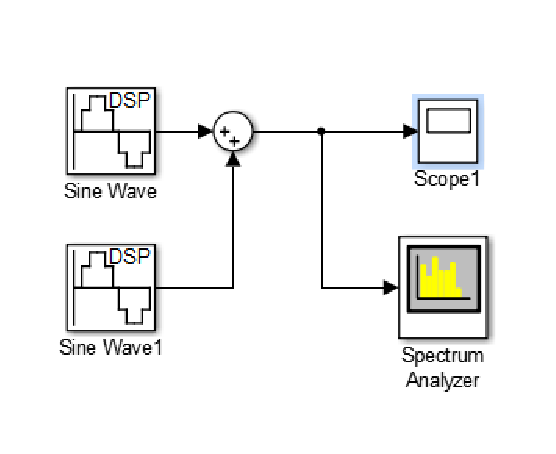
\includegraphics[width=10cm]{1_simulink} 
\caption{Полигармонический сигнал (Simulink)} 
\label{fig.l5_1s} 
\end{figure}
\begin{figure}[h]
\centering
\includegraphics[width=10cm]{lab5_1_simulink} 
\caption{Полигармонический сигнал} 
\label{fig.l5_2s1} 
\end{figure}
\begin{figure}[h]
\centering
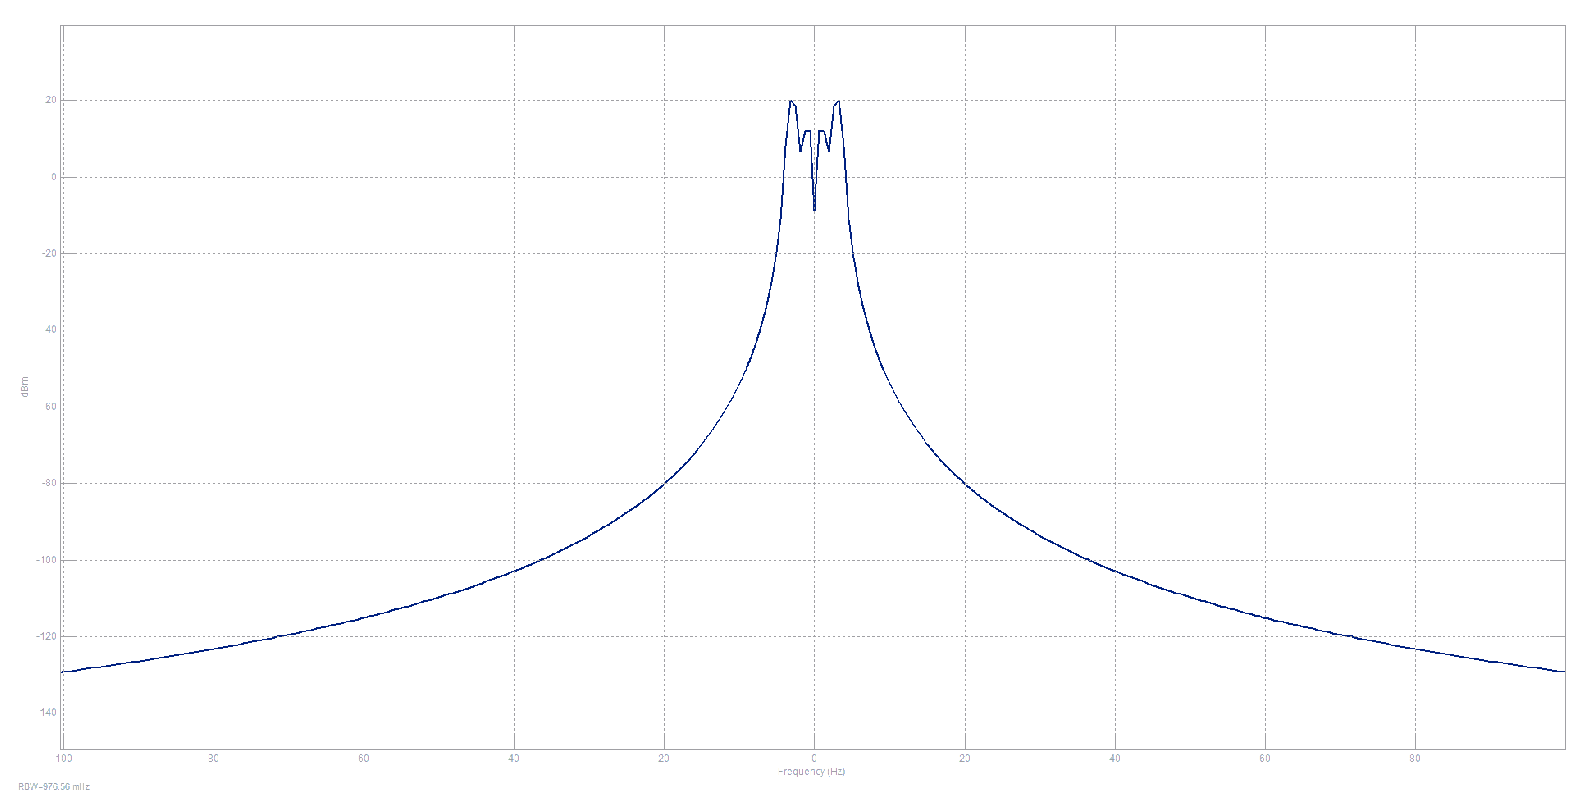
\includegraphics[width=10cm]{lab5_2_simulink}
\caption{Спектр полигармонического сигнала} 
\label{fig.l5_3s} 
\end{figure}

\item Прямоугольный импульсный сигнал (Рис. 14 - 16)
\begin{figure}[h]
\centering
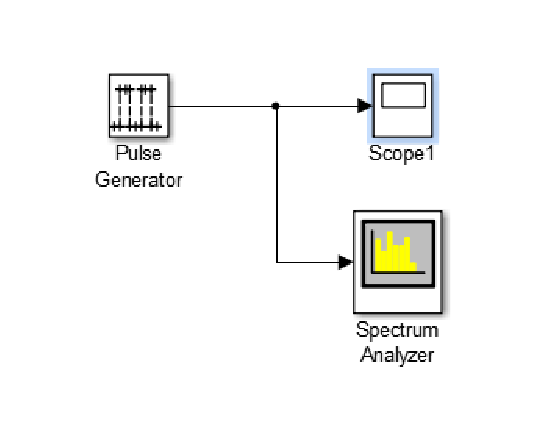
\includegraphics[width=10cm]{3_simulink} 
\caption{Прямоугольный импульсный сигнал (Simulink)} 
\label{fig.l5_4s} 
\end{figure}
\begin{figure}[h]
\centering
\includegraphics[width=10cm]{lab5_3_simulink} 
\caption{Прямоугольный импульсный сигнал} 
\label{fig.l5_5s} 
\end{figure}
\begin{figure}[h]
\centering
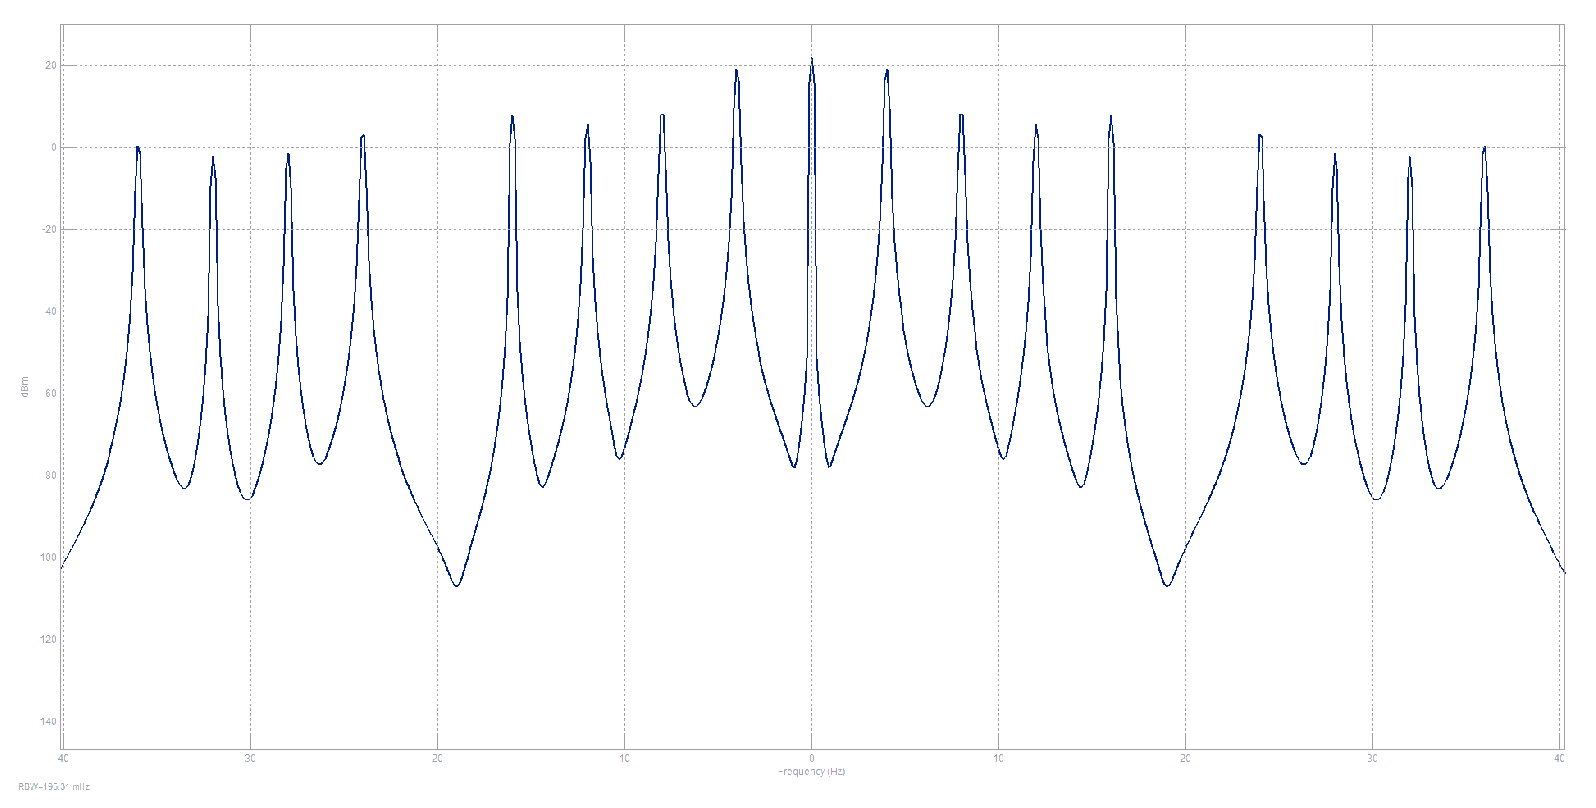
\includegraphics[width=10cm]{lab5_4_simulink}
\caption{Спектр прямоугольного сигнала} 
\label{fig.l5_6s} 
\end{figure}

\item Треугольный импульсный сигнал (Рис. 17 - 19)
\begin{figure}[h]
\centering
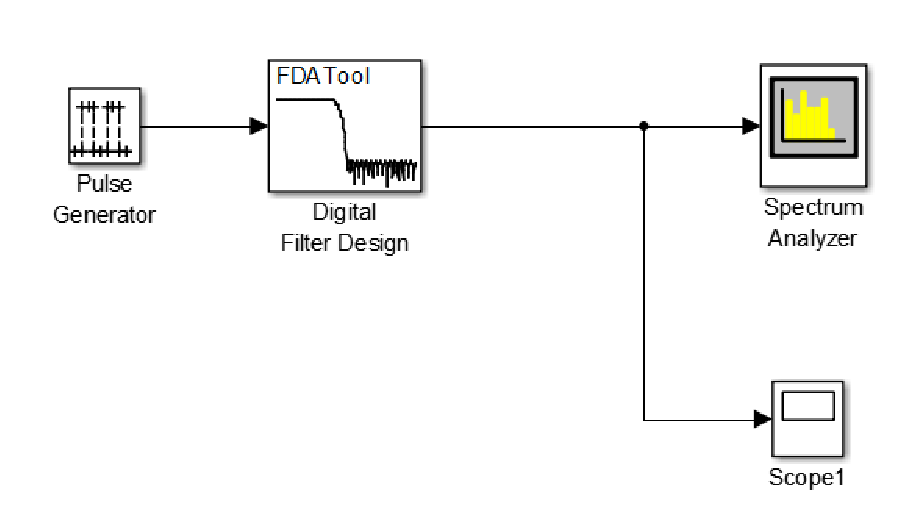
\includegraphics[width=10cm]{4_simulink} 
\caption{Треугольный импульсный сигнал (Simulink)} 
\label{fig.l5_7s} 
\end{figure}
\begin{figure}[h]
\centering
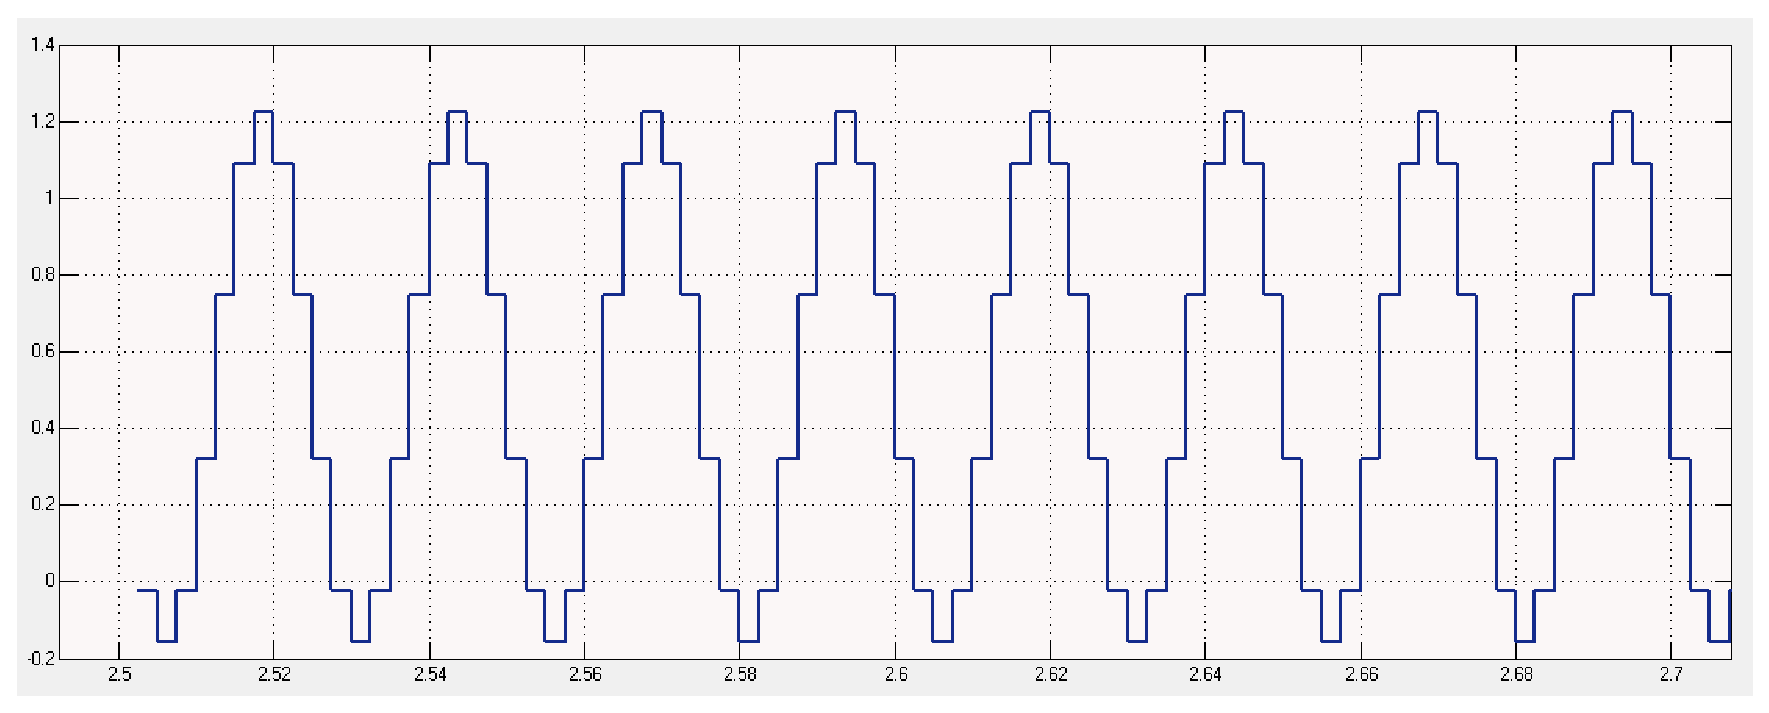
\includegraphics[width=10cm]{lab5_5_simulink} 
\caption{Треугольный импульсный сигнал} 
\label{fig.l5_8s} 
\end{figure}
\begin{figure}[h]
\centering
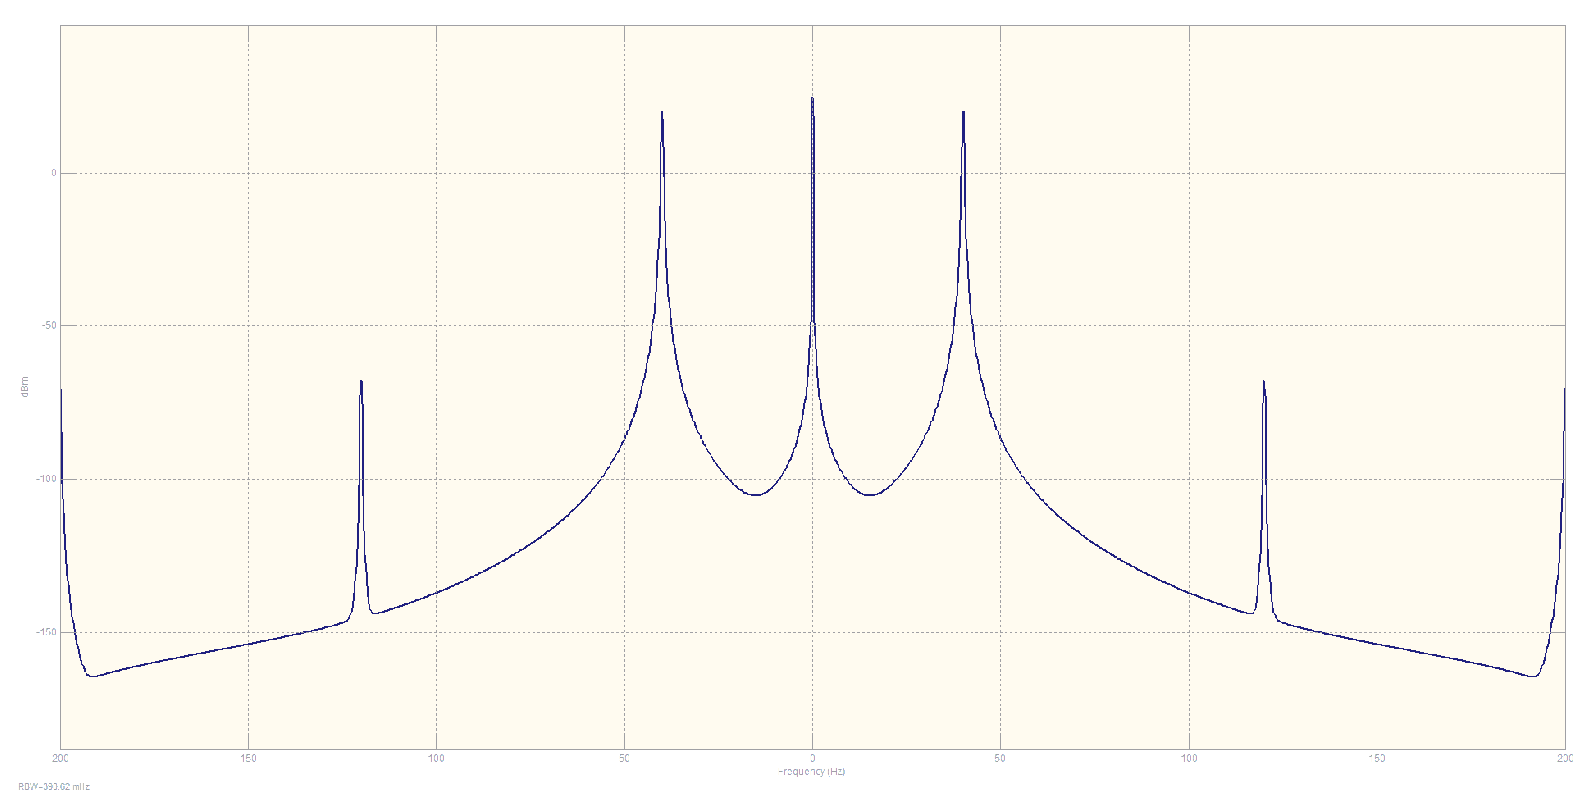
\includegraphics[width=10cm]{lab5_6_simulink}
\caption{Спектр треугольного сигнала} 
\label{fig.l5_9s} 
\end{figure}
\end{itemize}
\subsection{Выводы}
В результате проделанной работы было проведено моделирование в среде MatLAB и Simulink полигармонического, прямоугольного и треугольного импульсных сигналаов, а также получены их спектры. В Simulink для получения генератора треугольного сигнала используется генератор прямоугольных импульсов каскадно с фильтром с прямоугольным окном. Это обоснуется тем, что свертка двух прямоугольных импульсов в результате дает треугольный 
\end{document}